\section{Ячейка Фейстеля}
\selectlanguage{russian}

Одним из основных методов построения современных блоковых шифров является ячейка \textbf{Фейстеля} (Feistel), изображенная на рисунке~\ref{fig:Feistel}. Главная особенность шифрования с ячейкой Фейстеля состоит в том, что обратимость шифрования (т.~е. расшифрование) не зависит от обратимости преобразования $F$ внутри ячейки. Широкое применение ячеек Фейстеля в шифрах 1970--90-х годов вызвано бурным развитием персональных компьютеров. Шифрование выполняется \textbf{раундами}, на каждом раунде выполняется одно и то же преобразование ячейки Фейстеля, но с разными ключами. Общее количество раундов 16--32.

\begin{figure}[!ht]
    \centering
    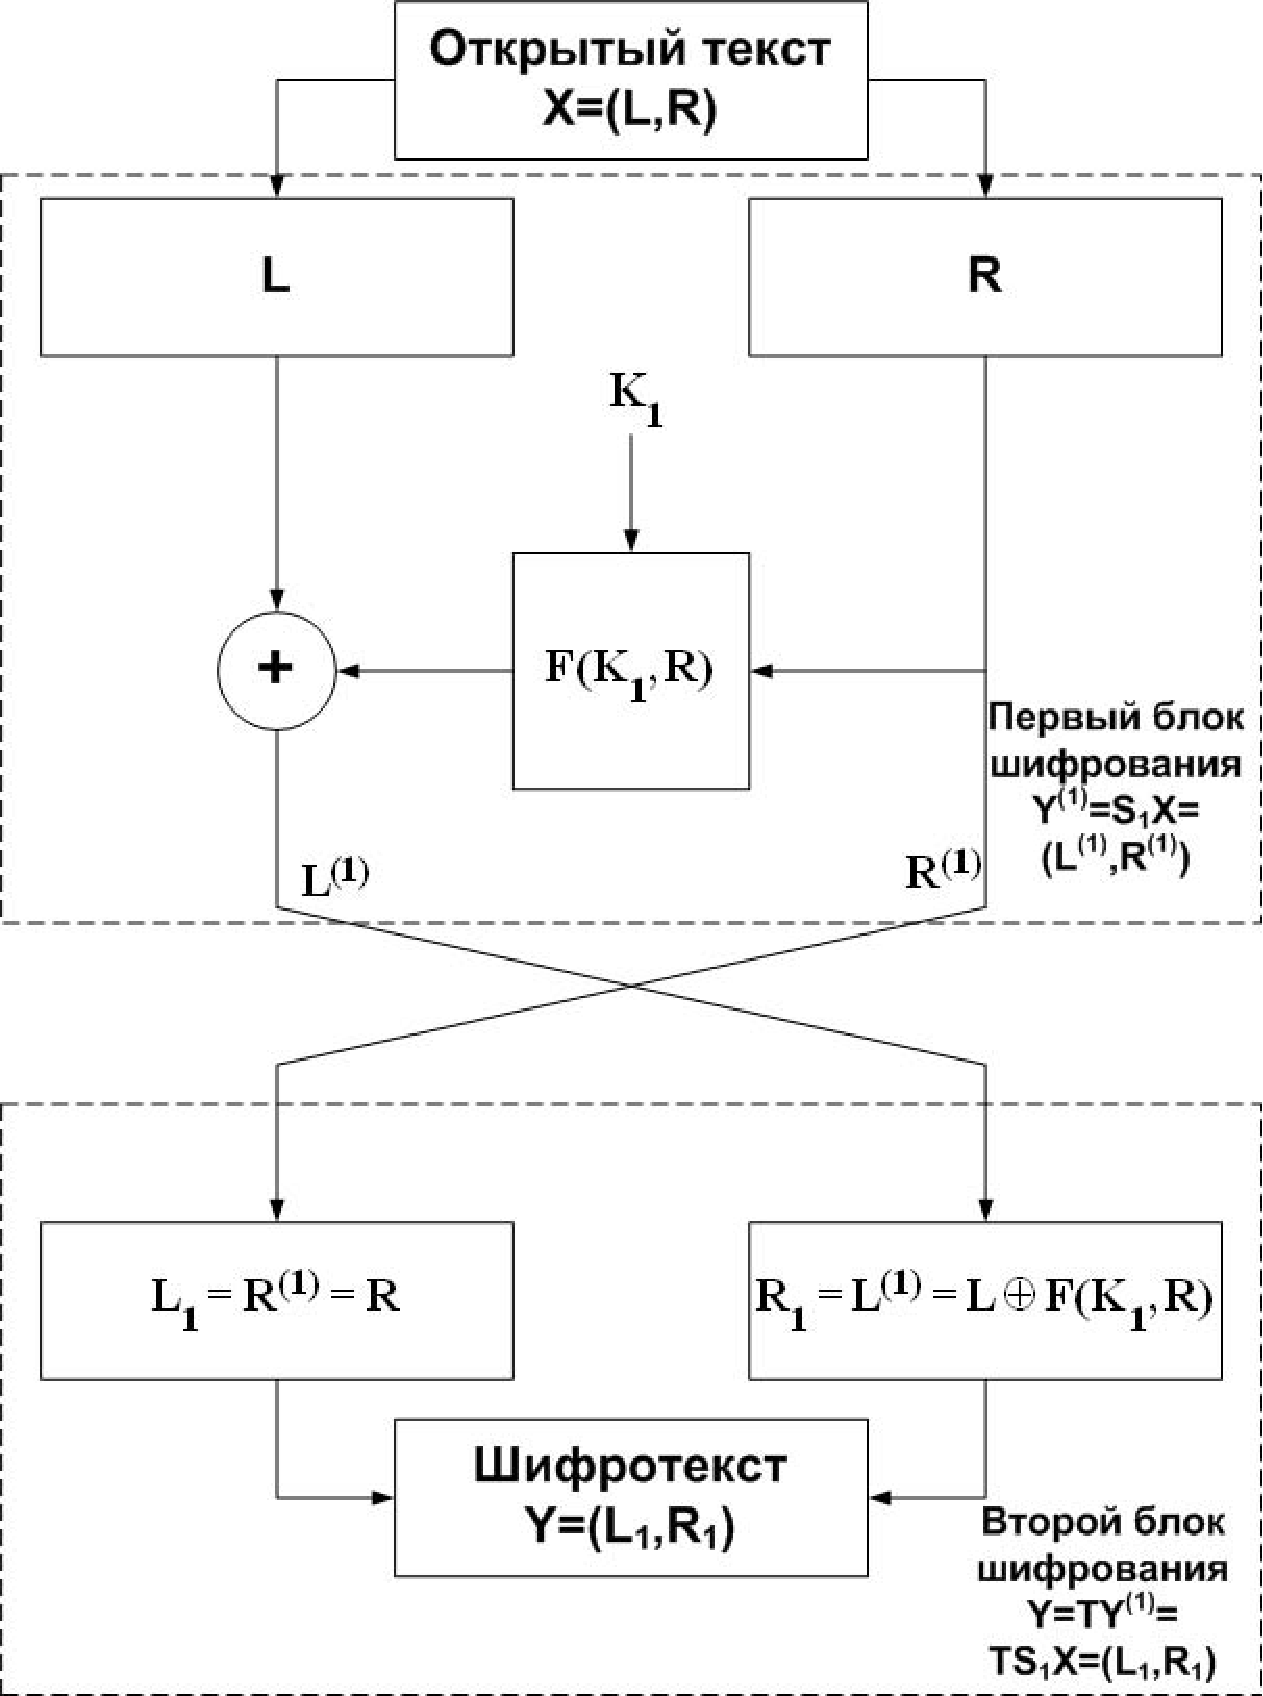
\includegraphics[width=0.6\textwidth]{pic/feistel}
    \caption{Ячейка Фейстеля\label{fig:Feistel}}
\end{figure}

Здесь введены обозначения: $X$ -- блок двоичных символов, который записан в регистр памяти, состоящий из двух частей, $X = (L,R)$, где $L$ -- начальное содержимое левого регистра, $\tilde{L}$ -- содержимое левого регистра сдвига после преобразования, $R$ -- начальное содержимое правого регистра, $\tilde{R}$ -- содержимое правого регистра после преобразования, $K$ -- ключ шифрования, задающий преобразование $F(K,R)$. Знак $\oplus$ определяет операцию побитового суммирования по модулю 2, то есть операцию XOR. Перекрёстные линии указывают на замену частей регистра. После одного элементарного преобразования содержимое правого регистра заменяется содержимым левого регистра и наоборот. $\tilde{L},\tilde{R}$ -- результат элементарного шифрования, выполненного за один раунд. $L_{1}$ -- содержимое правого регистра после замены, $R_{1}$ -- содержимое левого регистра после замены. Основным шифрующим преобразованием является функция $F$.

Ячейка Фейстеля -- произведение двух перестановок $T$ и $G$, где $T$ -- замена левой части на правую и наоборот. Запишем преобразование $Y=TG(X,L)$, выполняемое этой ячейкой:
\[
  \begin{array}{l}
    \tilde{X} = (\tilde{L}, \tilde{R}) = (L \oplus F(K,R), R) \equiv G(X, L), \\
    Y = TGX. \\
  \end{array}
\]

Если дважды применим перестановку, то получим снова открытый текст:
\[
    \begin{array}{l}
        \tilde{\tilde{L}} = \tilde{L} \oplus F(K, \tilde{R}) = (L \oplus F(K,R) \oplus F(K,R)) = L, \\
        \tilde{\tilde{R}} = R.\\
    \end{array}
\]

Многократное применение преобразования $Y=TG(X,L)$ с различными ключами представим в виде:
\[
  \begin{array}{l}
    Y_1 = T G_1 X,\\
    Y_2 = T G_2 Y_1 = T G_2 T G_1 X, \\
    \ldots, \\
    Y_{m-1} = T G_{m-1} Y_{m-2} = T G_{m-1} T G_{m-2} \ldots T G_1 X.\\
  \end{array}
\]
В первом уравнении показан результат первого шифрования с ключом $K_{1}$, во втором уравнении -- результат шифрования с ключом $K_{2}$ и т.~д., в $(m-1)$-м уравнении -- результат с ключом $K_{m-1}$. В последнем, $(m)$-м уравнении, перестановку $T$ можно не использовать:
\[
   Y_{m}= G_{m} Y_{m-1} = G_{m} T G_{m-1} \ldots T G_{1} X.\\
\]

Как видно из приведённых соотношений, пара величин -- содержимое регистра и первый ключ $X, K_{1}$ -- влияет на все позиции шифрованного текста. Полностью разрушается статистическая структура исходного текста за счёт преобразований, вызывающих \emph{лавинный эффект}\index{лавинный эффект}. \textbf{Лавинный эффект} -- это распространение <<влияния>> одного бита открытого текста (или ключа) на все остальные биты шифруемого блока за определённое количество раундов.
%Для ячеек Фейстеля это количество равно 2.

Одной из характеристик блокового шифра является число раундов, за которое достигается полная диффузия (конфузия) -- зависимость всех битов выхода (входа) от всех битов входа (выхода). Вход -- это открытый текст и ключ.

Криптостойкость ячейки Фейстеля подтверждается тем фактом, что не существует примеров её взлома (в случае шифра DES взлом был сделан полным перебором 56-битового ключа, а не взломом самой криптосистемы; например, российский стандарт ГОСТ 28147-89 на ячейке Фейстеля с 256-битовым ключом не взломан).

Рассмотрим процедуру расшифрования. Легальный пользователь знает все ключи и последовательность их применения. Он выполняет следующие операции. Имеем шифрованное сообщение $Y_{m}$. На первом шаге вычисляет
\[
    G_{m} Y_{m} = G_{m} G_{m} Y_{m-1} = Y_{m-1}.
\]
На втором шаге использует найденное сообщение $Y_{m-1}$ и аналогично находит $Y_{m-2}$:
\[
    G_{m-1} T Y_{m-1} = G_{m-1} T T G_{m-1} Y_{m-2} = Y_{m-2}.
\]
Продолжает этот процесс до получения $Y_{1}$. После этого находит $X$:
\[
    G_{1} T Y_{1} = G_{1} T T G_{1} X = X.
\]
Как показали эти операции, вычислительная сложность устройства расшифрования ячейки Фейстеля такая же, как сложность устройства шифрования.

Раундовые блоковые шифры должны обеспечивать \emph{диффузию}, при которой каждый бит входа и ключа влияет на все биты выхода, и \emph{конфузию}, при которой каждый бит выхода нелинейно зависит от всех битов входа и ключа.

Основные свойства, которыми должна обладать функция $F$:
\begin{itemize}
    \item создание лавинного эффекта,
    \item нелинейность по отношению к операции XOR.
\end{itemize}

Как правило, функция $F$ включает таблицы перестановки $P$ и подстановки групп бит, так называемые s-блоки (от слова substitution), и функцию перестановки, перемешивающую биты между последовательно исполняемыми $s$-блоками. В совокупности эти действия и обеспечивают требуемые свойства ячейки.
